% Minimal example paper for the LaTeX to Word converter.
\documentclass[12pt,a4paper]{article}
\usepackage[utf8]{inputenc}
\usepackage[T1]{fontenc}
\usepackage{amsmath}
\usepackage{amssymb}
\usepackage{amsthm}
\newtheorem{lemma}{Lemma}
\usepackage{graphicx}
\graphicspath{{figures/}}
\usepackage{booktabs}
\usepackage{algorithm}
\usepackage[noend]{algpseudocode}
\usepackage{hyperref}

\title{A Minimal Example Paper}
\author{Example Author}
\date{\today}

\begin{document}
\maketitle

\begin{abstract}
This short paper exists only to demonstrate the LaTeX to Word converter. It uses
numbered equations, two pseudocode algorithms with pruning (Apriori frequent-itemset
mining and association-rule generation), a lemma, a figure, a table, cross
references to all of them, and two citations.
\end{abstract}

\section{Introduction}
Sequential data mining has many applications \cite{Smith2020}. A common baseline
is the algorithm of \cite{Jones2018}, which we revisit in Section~\ref{sec:method}.

\section{Method}
\label{sec:method}
Let $D$ be a set of transactions over a set of items $I$. The support of an
itemset $X \subseteq I$ is the fraction of transactions that contain it:
\begin{equation}
\label{eq:support}
\mathrm{supp}(X) = \frac{|\{t \in D : X \subseteq t\}|}{|D|}.
\end{equation}
For an association rule $X \Rightarrow Y$, the confidence is the conditional
support
\begin{equation}
\label{eq:conf}
\mathrm{conf}(X \Rightarrow Y) = \frac{\mathrm{supp}(X \cup Y)}{\mathrm{supp}(X)}.
\end{equation}

\begin{lemma}[Apriori pruning]
\label{lem:apriori}
If an itemset $X$ is frequent, then every subset $X' \subseteq X$ is also frequent.
Equivalently, if any $(k-1)$-subset of a candidate $k$-itemset is infrequent, the
candidate cannot be frequent and may be pruned without computing its support.
\end{lemma}

Algorithm~\ref{alg:apriori} mines all frequent itemsets using the support of
Eq.~\eqref{eq:support} and the pruning rule of Lemma~\ref{lem:apriori}.

\begin{algorithm}
\caption{Apriori frequent-itemset mining}
\label{alg:apriori}
\begin{algorithmic}[1]
\Require transactions $D$, minimum support $\sigma$
\Ensure all frequent itemsets $\mathcal{F}$
\State $L_1 \gets \{\,\{i\} : i \in I,\ \mathrm{supp}(\{i\}) \ge \sigma\,\}$
\State $\mathcal{F} \gets L_1$; \ $k \gets 2$
\While{$L_{k-1} \neq \varnothing$}
    \State $C_k \gets \Call{AprioriGen}{L_{k-1}}$ \Comment{join step}
    \For{each candidate $c \in C_k$}
        \If{some $(k-1)$-subset of $c$ is not in $L_{k-1}$}
            \State remove $c$ from $C_k$ \Comment{prune step (Lemma~\ref{lem:apriori})}
        \EndIf
    \EndFor
    \State $L_k \gets \{\, c \in C_k : \mathrm{supp}(c) \ge \sigma \,\}$
    \State $\mathcal{F} \gets \mathcal{F} \cup L_k$; \ $k \gets k + 1$
\EndWhile
\State \Return $\mathcal{F}$
\end{algorithmic}
\end{algorithm}

Given the frequent itemsets, Algorithm~\ref{alg:rules} derives the association
rules and prunes them with the confidence of Eq.~\eqref{eq:conf}.

\begin{algorithm}
\caption{Rule generation with confidence pruning}
\label{alg:rules}
\begin{algorithmic}[1]
\Require frequent itemsets $\mathcal{F}$, minimum confidence $\gamma$
\Ensure association rule set $\mathcal{R}$
\State $\mathcal{R} \gets \varnothing$
\For{each itemset $Z \in \mathcal{F}$ with $|Z| \ge 2$}
    \For{each non-empty proper subset $X \subset Z$}
        \State $Y \gets Z \setminus X$
        \If{$\mathrm{conf}(X \Rightarrow Y) \ge \gamma$}
            \State $\mathcal{R} \gets \mathcal{R} \cup \{X \Rightarrow Y\}$
        \Else
            \State prune every rule whose antecedent is a subset of $X$ \Comment{anti-monotone}
        \EndIf
    \EndFor
\EndFor
\State \Return $\mathcal{R}$
\end{algorithmic}
\end{algorithm}

\section{Experiments}
\label{sec:experiment}
We run Algorithm~\ref{alg:apriori} on a synthetic transaction database and vary the
minimum support $\sigma$. Figure~\ref{fig:runtime} shows that the runtime drops
sharply as $\sigma$ increases, because the pruning of Lemma~\ref{lem:apriori}
removes more candidates early. For comparison we also plot the FP-growth baseline
\cite{Han2000}.

\begin{figure}[ht]
\centering
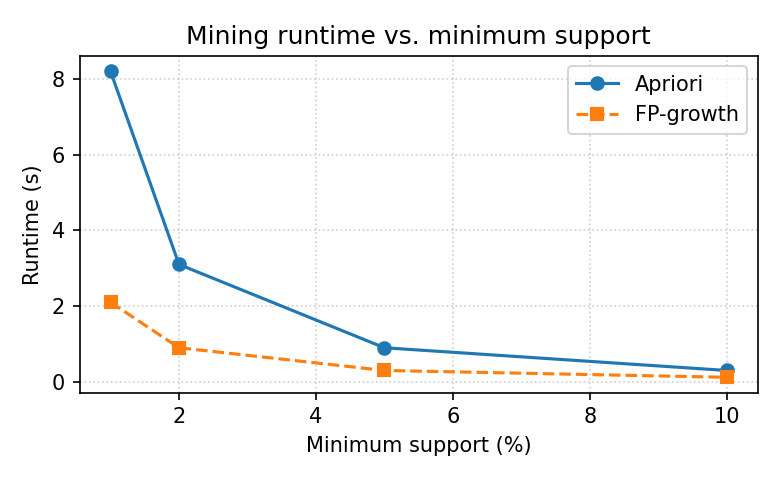
\includegraphics[width=0.7\linewidth]{runtime_apriori.png}
\caption{Mining runtime versus the minimum support threshold.}
\label{fig:runtime}
\end{figure}

Table~\ref{tab:results} reports, for each support threshold, the number of frequent
itemsets and association rules produced by Algorithm~\ref{alg:rules}.

\begin{table}[ht]
\centering
\caption{Frequent itemsets and rules found at each support threshold.}
\label{tab:results}
\begin{tabular}{rrr}
\toprule
\textbf{Support (\%)} & \textbf{Frequent itemsets} & \textbf{Rules} \\
\midrule
1  & 312 & 1045 \\
2  & 148 & 392 \\
5  & 47  & 86 \\
10 & 13  & 18 \\
\bottomrule
\end{tabular}
\end{table}

As summarised in Figure~\ref{fig:runtime} and Table~\ref{tab:results}, a higher
support threshold yields fewer patterns and faster mining, which matches the
pruning behaviour analysed in Section~\ref{sec:method}.


\bibliographystyle{IEEEtran}
\bibliography{references}
\end{document}
